\documentclass[a4paper,12pt]{article}
\usepackage[utf8]{ inputenc}
\usepackage[ngerman]{babel}
\usepackage[a4paper, left=2.5cm, right=2.5cm]{geometry}
\usepackage{graphicx}
\usepackage{subcaption}
\usepackage{fancyhdr}
\usepackage{pdfpages}
\usepackage{listings}
\usepackage{hyperref}
\usepackage[official]{eurosym}
\usepackage{float}

\pagestyle{fancy}
\lstset{
	language=Matlab,
	breaklines=true,
	morekeywords={matlab2tikz},
	keywordstyle=\color{blue},
	morekeywords=[2]{1}, keywordstyle=[2]{\color{black}},
	identifierstyle=\color{black},
	stringstyle=\color{mylilas},
	commentstyle=\color{mygreen},
	showstringspaces=false,
	mathescape=true
	emph=[1]{for,end,break},emphstyle=[1]\color{red},
}

\lhead{PV im Stromsystem – Strommarkt}
\chead{}
\rhead{Gruppe D}

\begin{document}
	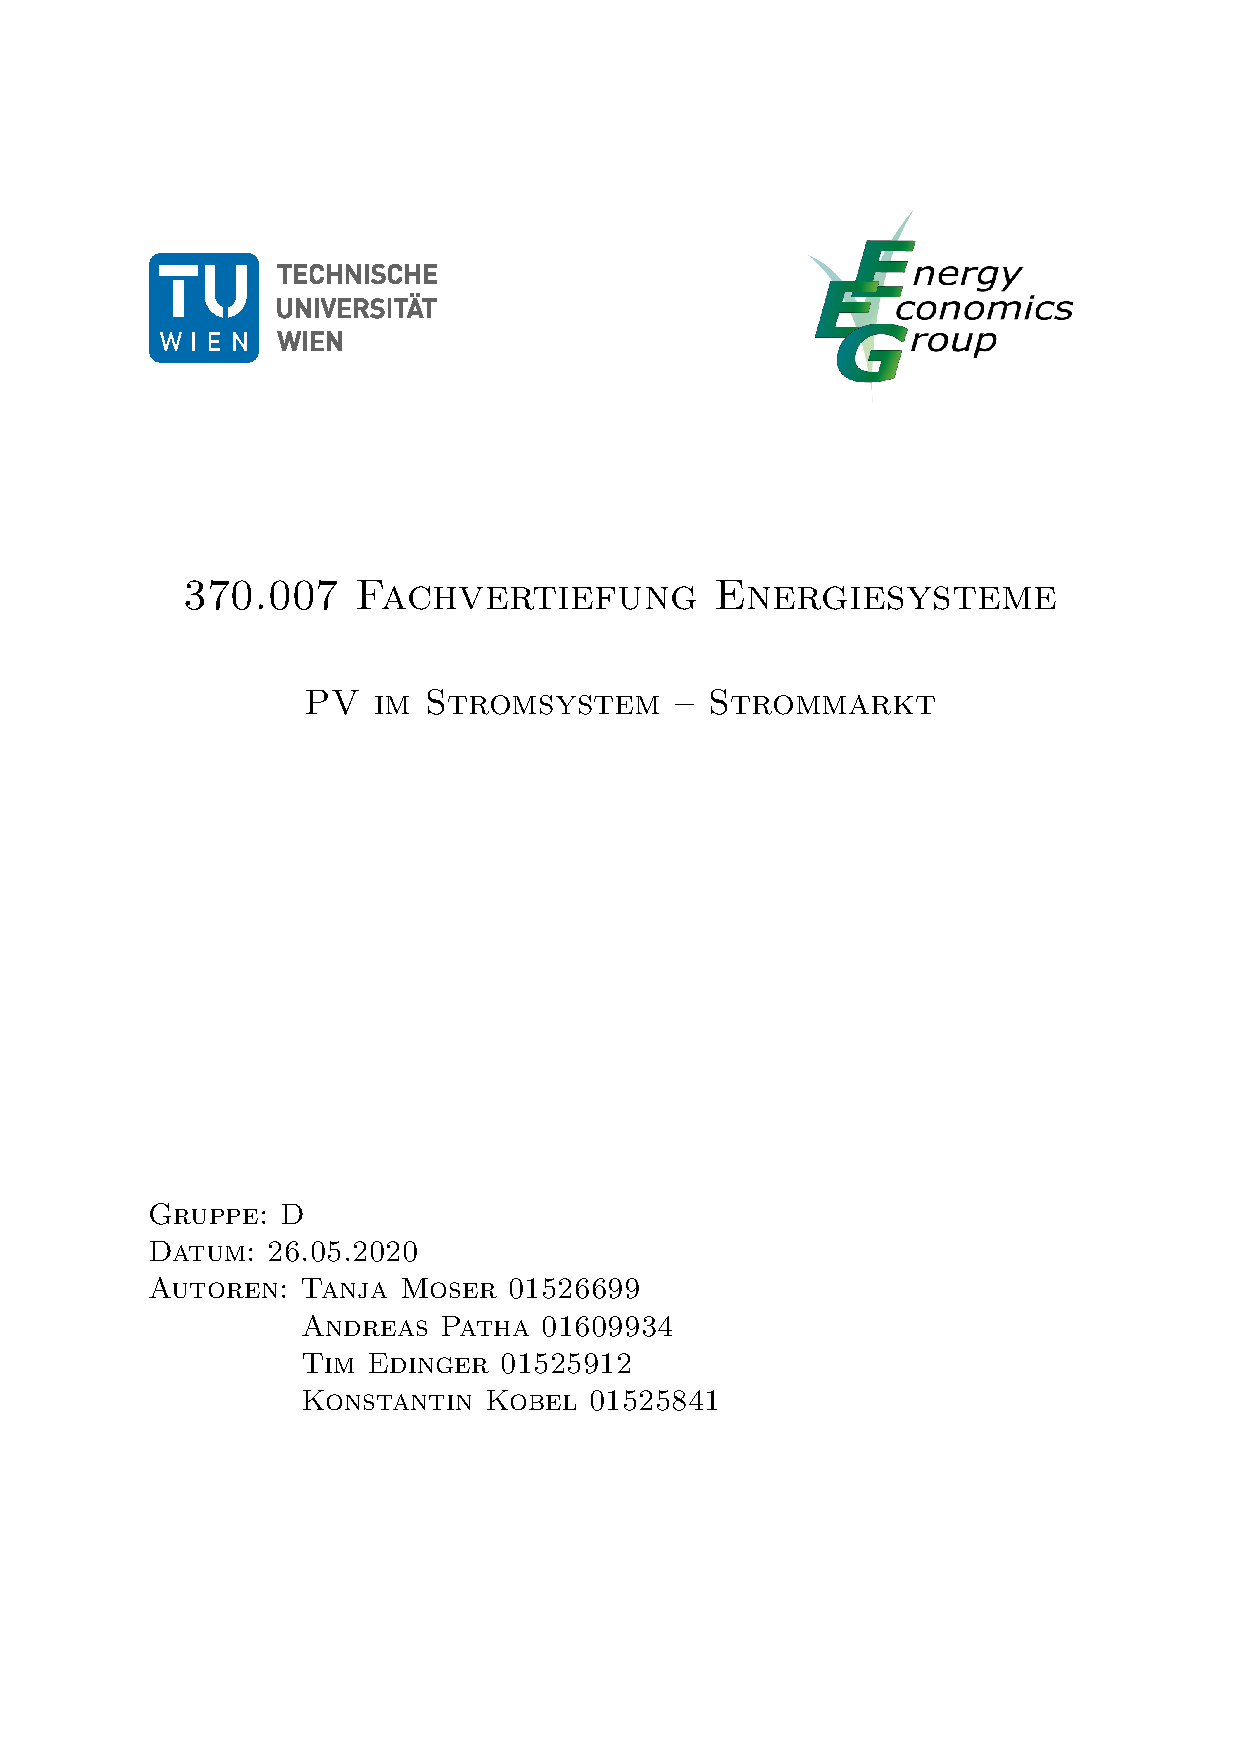
\includepdf{Protokoll_titlepage.pdf}

	\newpage
	\tableofcontents

	\newpage
	\section{Aufgabenstellung}
	\label{sec:Aufgabenstellung}
	In der vierten Übung sollen der Strommarkt und seine Entwicklung über die letzten Jahre, betrachtet werden. Besonders im Fokus stehen hierbei die Spotmarktpreise, die Stromerzeugung und die Netzlast, zu den unterschiedlichen Zeitpunkten.
	\subsection{Aufgabe 4.1}
	\label{sec:Aufgabenstellung41}
	In Aufgabe 4.1 sollen die Last und die Residuallast für das Marktgebiet Österreich/Deutschland, über ein Jahr, analysiert werden. Zusätzlich soll der Zusammenhang zwischen dem Spotmarktpreis und der Einspeisung von erneuerbaren Energien beleuchtet werden.\\ \par
	Folgende \textbf{Parameter} werden uns hierzu zur Verfügung gestellt:
	\begin{itemize}
		\item Die Datei $Load\_Production.mat$ beinhaltet die stündlichen Werte für die Netzlast (in $MW$) sowie die normierte PV-Erzeugung (in $MW/MW_{peak}$), über ein Jahr.
		\item In der Datei $Daten\_Preise\_Last\_2012.xlsx$ befinden sich stündliche Jahresdaten, aus dem Jahr 2012, zu der Netzlast, der Erzeugung durch PV- und Wind-Anlagen, sowie zu den Spotpreisen.
		\item Die Datei $Spotpreis.mat$ beinhaltet für die Jahre 2008 bis 2016 die mittleren stündlichen Spotmarktpreise, über das jeweilige Jahr, in $\mbox{\euro}/MWh$. Schaltjahre wurden bei $8760$ abgeschnitten.
	\end{itemize}
	\noindent Folgende \textbf{Aufgabenstellungen} sollen behandelt werden:
	\begin{itemize}
		\item[a)] Stellen Sie eine Dauerlinie der Last und der Residuallast ($Last - PV_{Produktion}$) für eine installierte Leistung von PV-Anlagen in der Höhe von 0 bis 200 GW dar. (in 50GW-Intervallen).\newline Was beobachten Sie?
		\item[b)] Betrachten Sie im Folgenden die tatsächlichen Daten der Erneuerbaren (Wind und PV) aus dem Jahr 2012. Stellen Sie die Last sowie Residuallast ($Last - PV_{Produktion} - Wind_{Produktion}$) als Leistungsdauerlinie dar.
		\item[c)] Erstellen Sie 3 Scatterplots (siehe Matlab-Funktion scatter) des Spotmarktpreises in Abhängigkeit von:
		\begin{itemize}
			\item Last
			\item Residuallast
			\item Einspeisung der Erneuerbaren
		\end{itemize}
		\item[d)] Wie interpretieren Sie die Scatterplots? Decken sich die Ergebnisse mit ihren Erwartungen?
	\end{itemize}
	\subsection{Aufgabe 4.2}
	\label{sec:Aufgabenstellung42}
	Das Ziel von Aufgabe 4.2 ist es die historische Entwicklung der Großhandelsstrompreise vom Jahr 2008 bis zum Jahre 2016 zu beschreiben.\\ \par
	\noindent	Die hierfür nötigen \textbf{Parameter} können dem Kapitel \hyperref[sec:Aufgabenstellung41]{Aufgabe 4.1} entnommen werden.\\ \par
	\noindent Die \textbf{Aufgaben} lauten:
	\begin{itemize}
		\item[a)] Erstellen Sie die Preisdauerlinie für die Jahre 2008 bis 2016.\newline Was beobachten Sie?
		\item[b)] Erstellen Sie eine Grafik der mittleren stündlichen Großhandelsstrompreise für alle 24h für die Jahre 2016 und 2008. Sprich für jede Stunde soll der Mittelwert aus 365 Tagen gebildet werden.
		\begin{itemize}
			\item Alternativ können Sie dies auch mit einem Boxplot darstellen.
			\item Was erkennen Sie daraus?
		\end{itemize}
	\end{itemize}
	\subsection{Aufgabe 4.3}
	\label{sec:Aufgabenstellung43}
	Aufgabe 4.3 befasst sich mit der Entwicklung des monetären Ertrags einer PV-Anlage, über die Jahre 2008 bis 2016.\\ \par
	\noindent Die dazu gegebenen \textbf{Parameter} sind folgende:
	\begin{itemize}
		\item Es wird von einer $1kWp$ PV-Anlage ausgegangen.
		\item Das Erzeugungsprofil der PV-Anlage ist in der Datei $Load\_PVProduction.mat$ enthalten.
	\end{itemize}
	Für den konkreten Fall aus Aufgabe 4.3 soll die Annahme getroffen werden, dass die komplette Erzeugung am Spotmarkt verkauft wird.\\ \par
	\noindent Speziell sollen folgende \textbf{Aufgaben} behandelt werden:
	\begin{itemize}
		\item[a)] Berechnen Sie den monetären Ertrag am Spotmarkt (Marktwert) einer $1kWp$-PV-Anlage für die Jahre 2008 bis 2016 (das PV-Erzeugungsprofil (in $MW/MW_{peak}$) finden Sie im File $Load\_PVProduction.mat$)
		\item[b)] Geben Sie die monetären Erträge (der $1kWp$-Anlage) der Tage 4 bis 34 und 180 bis 220 im Jahr 2008 und 2016 an.
		\item[c)] Wie interpretieren Sie die jährliche Entwicklung der Erträge? Was schließen Sie aus den Ergebnissen?
	\end{itemize}
	\newpage
	\section{Berechnungen}
	\label{sec:Berechnungen}
	\subsection{Last und Residuallast}
	Die \textbf{Last} bezeichnet in der elektrischen Energietechnik die gesamte, in einem Stromnetz nachgefragte, elektrische Leistung. \\ \par
	\noindent Die \textbf{Residuallast} bezeichnet in der elektrischen Energietechnik die in einem Stromnetz nachgefragte elektrische Leistung, abzüglich des Anteils fluktuierender Einspeisung von dargebotsabhängigen Erzeugern, wie Windkraft- oder PV-Anlagen. Die Residuallast ist demnach die Leistung, die von Regelkraftwerken gedeckt werden muss.\\ \par
	\noindent Die Berechnung der Residuallast erfolgt für den Fall aus \hyperref[sec:Aufgabenstellung41]{Aufgabe 4.1.a} wie folgt:
	\begin{equation}
	Residuallast = Last - PV_{Profil} * PV_{Leistung}
	\end{equation}
	\begin{itemize}
		\item \textbf{Last} ist die in der Datei $Load\_Production.mat$ zur Verfügung gestellte Netzlast.
		\item \textbf{PV-Profil} entspricht dem in der Datei $Load\_Production.mat$ enthaltenen Erzeugungsprofil einer PV-Anlage.
		\item \textbf{PV-Leistung} entspricht der installierten Leistung. Für den Fall aus \hyperref[sec:Aufgabenstellung41]{Aufgabe 4.1.a} soll die installierte Leistung von $0GW$ bis $200GW$, in $50GW$-Schritten variiert werden.
	\end{itemize}
	Im Falle von \hyperref[sec:Aufgabenstellung41]{Aufgabe 4.1.b} erfolgt die Berechnung der Residuallast über folgende Formel:
	\begin{equation}
	Residuallast = Last - PV_{Produktion} - Wind_{Produktion}
	\end{equation}
	\begin{itemize}
		\item \textbf{Last} ist die in der Datei $Daten\_Preise\_Last\_2012.xlsx$ zur Verfügung gestellte Netzlast, für das Jahr 2012.
		\item \textbf{PV-Produktion} entspricht der in der Datei $Daten\_Preise\_Last\_2012.xlsx$ enthaltenen PV-Einspeisung, für das Jahr 2012.
		\item \textbf{Wind-Produktion} entspricht der in der Datei $Daten\_Preise\_Last\_2012.xlsx$ enthaltenen Einspeisung aus Windkraft-Anlagen, für das Jahr 2012.
	\end{itemize}
	\newpage
	\subsection{Monetärer Ertrag einer 1kWp PV-Anlage}
	Der monetäre Ertrag einer PV-Anlage ergibt sich aus der Multiplikation der Kraftwerkleistung, den Profilwerten und dem jeweiligen Spotpreis. Durch Aufsummieren der einzelnen Werte eines Jahres, erhält man den gesamten monetären Ertrag des jeweiligen Jahres (in Euro).
	\begin{equation}
	Ertrag(a) = \sum\nolimits_{i=1}^n PV_{Leistung} * PV_{Profil,k} * Spotpreis_k(a)
	\end{equation}
	\begin{itemize}
		\item \textbf{Ertrag} entspricht dem gesamten monetären Ertrag eines Jahres, in Euro.
		\item \textbf{a} ist das entsprechende Jahr, für das der monetäre Ertrag errechnet werden soll. (in unserem Fall von 2008 bis 2016)
		\item \textbf{k} entspricht dem Intervall, in dem Daten vorhanden sind (in unserem Fall handelt es sich um stündliche Daten. Daraus folgt, dass \textbf{n} einem Wert von 8760 Stunden entspricht.).
		\item \textbf{PV-Leistung} ist die installierten Leistung der PV-Anlage. Für den Fall aus \hyperref[sec:Aufgabenstellung43]{Aufgabe 4.3} entspricht das $1kWp$.
		\item \textbf{PV-Profil} ist das Erzeugungsprofil der PV-Anlage.
		\item \textbf{Spotpreis} entspricht dem jeweiligen Spotpreis im Jahr $a$, zum Zeitpunkt $k$.
	\end{itemize}
	\newpage
	\section{Ergebnisse}
	\label{sec:Ergebnisse}
	\subsection{Aufgabe 4.1 - Last und Residuallast}
	\subsubsection{Aufgabe 4.1.a - Dauerlinie der Last und der Residuallast}
	Das Ziel von Aufgabe 4.1.a war es die Dauerlinie der Last darzustellen.\\ \par
	\noindent Die Daten für die Darstellung sind in der Datei $Load\_PVProduction.mat$ enthalten. Um eine korrekte Darstellung der Dauerlinie zu erhalten, müssen die Werte absteigend sortiert werden.\newline
	Folgender MATLAB Code sortiert die Daten, der in der Datei $Load\_PVProduction.mat$ enthaltenen Variable $Last$ und plottet sie.
	\begin{lstlisting}
	plot(sort(Last, "descend"));
	\end{lstlisting}
	Der deraus resultierende Graph ist in Abbildung 1 dargestellt.
	\begin{figure}[H]
		\centering
		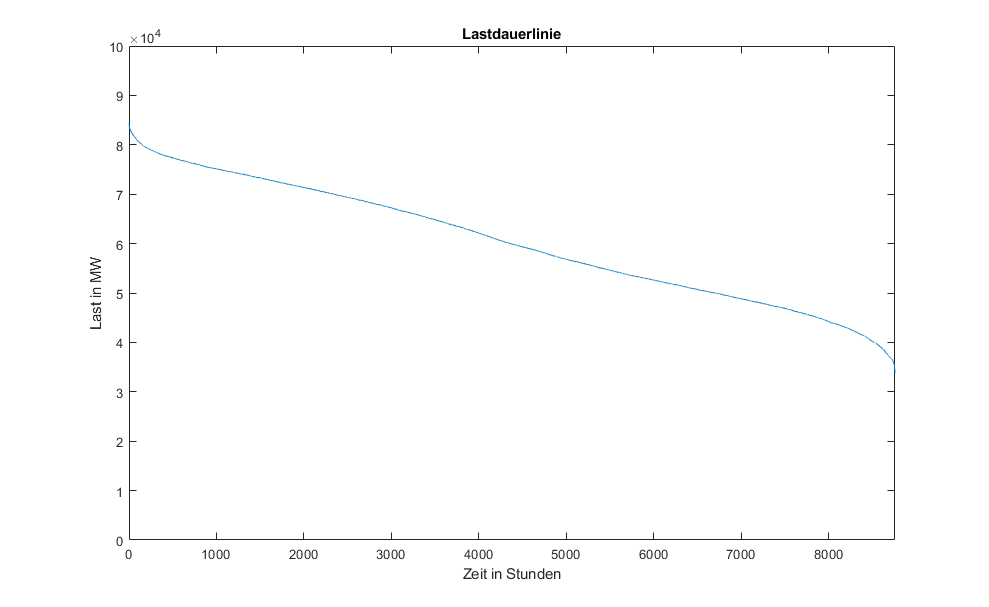
\includegraphics[width=12cm]{img/results/Lastdauerlinie}
		\caption{Dauerlinie der Last.}
	\end{figure}
	\noindent Zusätzlich sollte in Aufgabe 4.1.a die Residuallast, in Abhängigkeit von der installierten Leistung von PV-Anlagen, ermittelt werden.\\
	Hierzu soll von einer installierten Leistung von $0$ bis $200GW$ ausgegangen werden. Die installierte Leistung soll in Intervallen von $50GW$ erhöht werden.\\
	Folgender MATLAB Code erzeugt mit Hilfe der Variablen $Last$ und $PV_profil$ aus der Datei $Load\_PVProduction.mat$ sowie der Variable $iLeistung$, welche für die installierte Leistung steht, das in Abbildung 2 dargestellte Diagramm.
	\begin{lstlisting}
	iLeistung = 0:50:200;

	for l=1:length(iLeistung)
		Residuallast = Last $-$ (PV_profil .* (iLeistung(l) * 1000));
		plot(sort(Residuallast, "descend"))
		hold on
	end
	\end{lstlisting}
	\begin{figure}[H]
		\centering
		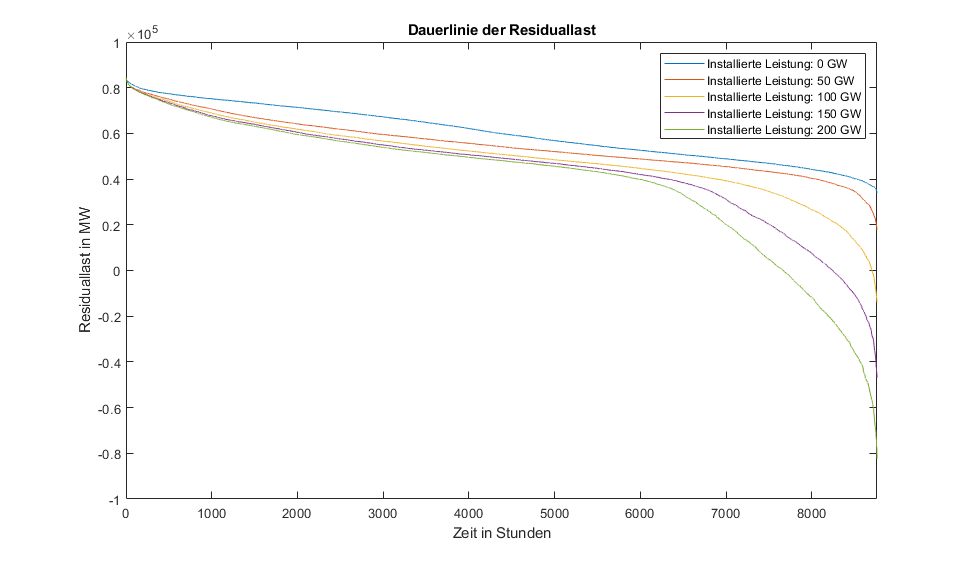
\includegraphics[width=12cm]{img/results/DauerlinieResiduallast}
		\caption{Dauerlinie der Residuallast, in Abhängigkeit der installierten Leistung von PV-Anlagen.}
	\end{figure}
	Wie man an dem Graphen erkennen kann, sinkt mit zunehmender installierter Leistung die Residuallast. Das bedeutet, dass ein geringerer Anteil der Last auf Regelkraftwerke abfällt und demnach eine höhere gesamte Last abgedeckt werden kann.\\ Jedoch ist auch ersichtlich, dass selbst die Einspeisung von PV-Anlagen mit einer installierten Leistung von $200GW$ in den ersten $1000$ Stunden (circa ein Achtel des Jahres) kaum eine Einfluss auf die Residuallast haben.\\
	In den letzten $1000$ Stunden des Jahres sorgt die geringere Last jedoch dafür, dass die Residuallast teilweise in den negativen Bereich fällt. Der Grund hierfür ist der geringere Stromverbrauch im Sommer, da Verbraucher wie die Beleuchtung oder Heizung nicht aktiv sind. Gleichzeitig ist die Erzeugung bei PV-Anlagen am höchsten.\\
	Gegenteiliges Verhalten (wenig Erzeugung, hohe Last) kann im Winter beobachtet werden.\\
	Diesem Problem kann mit ausreichendem Speichern von Energie, im Sommer (zum Beispiel in Pumpspeicherkraftwerken), entgegengewirkt werden.
	\subsubsection{Aufgabe 4.1.b - Dauerlinie der Last und der Residuallast für das Jahr 2012}
	In Aufgabe 4.1.b sollten die tatsächlichen Dauerlinien für die Last und die Residuallast, für das Jahr 2012, dargestellt werden. In dieser Aufgabe sollte ebenfalls die Erzeugung durch Windkraft-Anlagen berücksichtigt werden.\\ \par
	\noindent Mit Hilfe der in der Datei $Daten\_Preise\_Last\_2012.xlsx$ enthaltenen Daten zur Netzlast, der PV- und der Wind-Erzeugung, kann die Dauerlinie analog zu Aufgabe 4.1.a erstellt werden:
	\begin{lstlisting}
	plot(sort(Netzlast2012, "descend"))
	\end{lstlisting}
	Die Variable $Netzlast2012$ entspricht den in der Datei $Daten\_Preise\_Last\_2012.xlsx$ enthaltenen Daten für die Last.\\
	Abbildung 3 zeigt die resultierende Dauerlinie der Last, für das Jahr 2012.
	\begin{figure}[H]
		\centering
		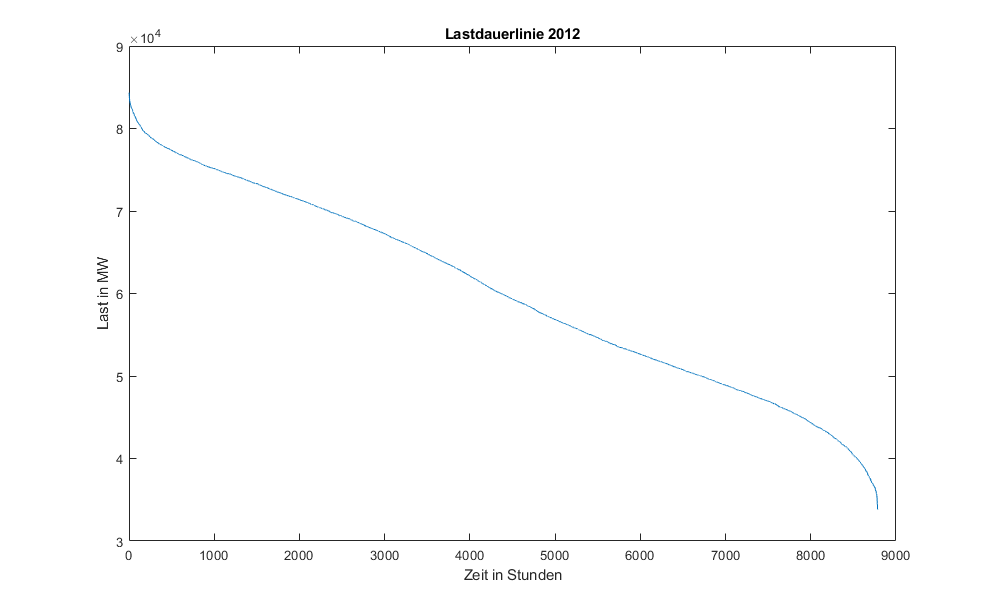
\includegraphics[width=12cm]{img/results/Lastdauerlinie2012}
		\caption{Die Dauerlinie der Last, für das Jahr 2012.}
	\end{figure}
	Mithilfe der in der Datei $Daten\_Preise\_Last\_2012.xlsx$ zur Verfügung gestellten Variablen $PV2012$, welche die PV-Erzeugung über das Jahr 2012 abbildet und $Wind2012$, welche die Erzeugung aus der Windkraft darstellt, kann die Dauerlinie der Residuallast, für das Jahr 2012, ermittelt werden.\\
	Das Resultat ist in Abbildung 4 dargestellt.
	\begin{figure}[H]
		\centering
		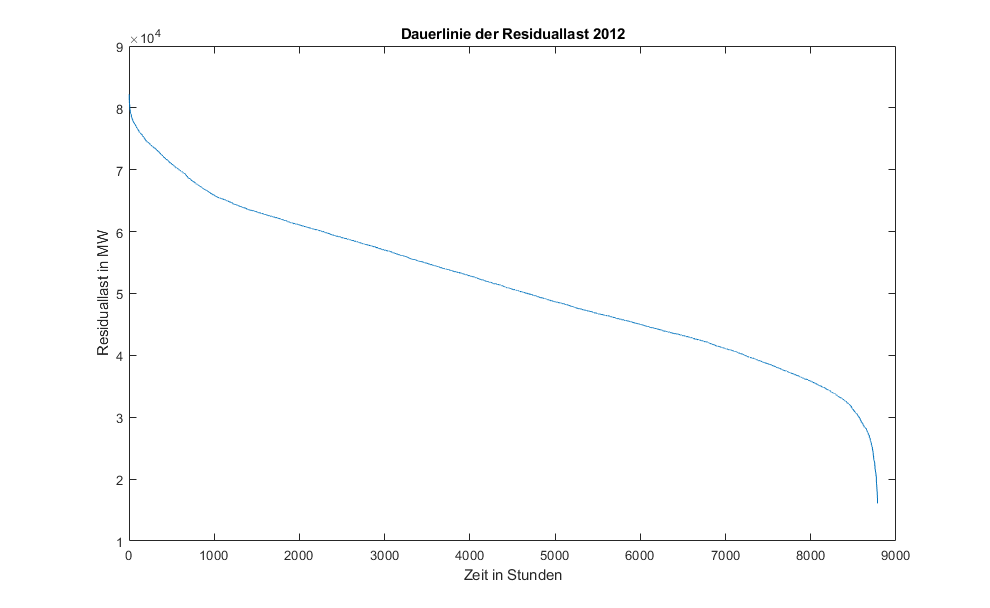
\includegraphics[width=12cm]{img/results/DauerlinieResiduallast2012}
		\caption{Die Dauerlinie der Residuallast für das Jahr 2012.}
	\end{figure}
	Der Vergleich der beiden Diagramme zeigt, dass die Dauerlinie der Residuallast, im Vergleich zur Dauerlinie der Last, in den ersten $1000$ Stunden des Jahres stärker abfällt. Zwischen $1000$ Stunden und $8000$ Stunden ist die Kurve der Residuallast flacher, als die Kurve der Last. In den letzten $760 Stunden$ fällt die Kurve der Residuallast noch einmal sehr steil ab.\\
	Der Vergleich zeigt, dass mit Hilfe der Erzeugung durch erneuerbare Energien die Stunden, in denen eine hohe Leistung von Regelkraftwerken abgedeckt werden muss (über $70.000 MW$), reduziert werden kann (auf ungefähr $1000$ Stunden). Zeitweise sinkt die Residuallast sogar auf nur circa $15.000MW$.
	\subsubsection{Aufgabe 4.1.c - Abhängigkeiten des Spotmarktpreises}
	In Aufgabe 4.1.c sollte die Abhängigkeit der Spotmarktpreise, des Jahres 2012, von der Netzlast, der Residuallast und der Einspeisung erneuerbarer Energien dargestellt werden.\\
	Die Interpretation der Ergebnisse findet sich in Kapitel \hyperref[sec:Ergebnisse41d]{Aufgabe 4.1.d - Interpretation der Scatter-Plots}.\\ \par
	\noindent Zum Erstellen eines Scatter-Plots ist folgender MATLAB Code notwendig:
	\begin{lstlisting}
	scatter(Netzlast2012, Spotpreis2012)
	\end{lstlisting}
	Die Variablen $Netzlast2012$ und $Spotpreis2012$ wurden in der Datei $Daten\_Preise\_Last\_2012.xlsx$ zur Verfügung gestellt. Die Variable $Netzlast2012$ wird für die beiden weiteren Diagramme durch die die Variablen $Residuallast2012$ und $EinspeisungErneuerbareEnergie2012$ ersetzt.\\
	Die resultierenden Scatter-Plots sind in den Abbildungen 5-7 dargestellt.
	\begin{figure}[H]
		\centering
		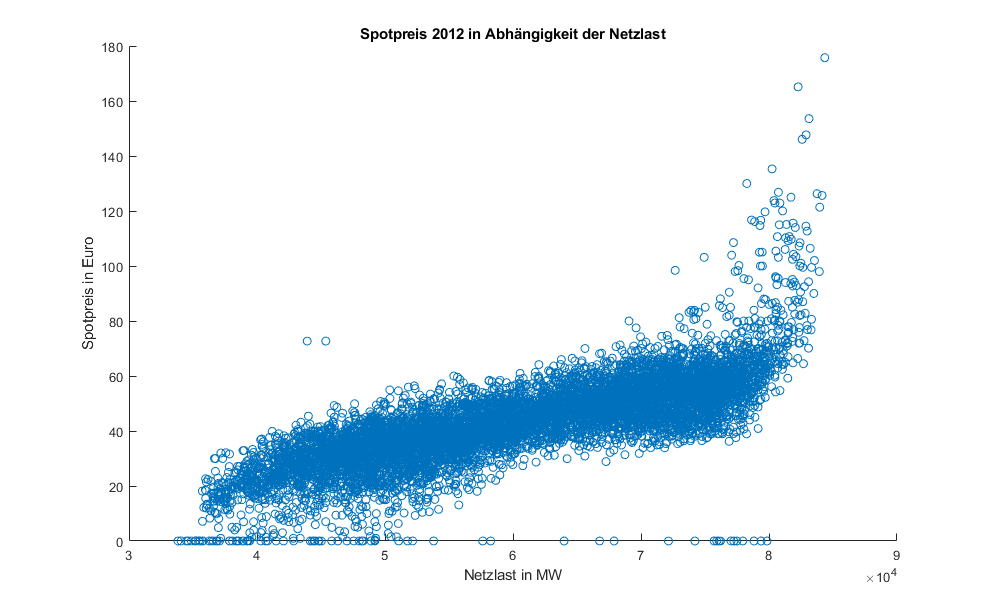
\includegraphics[width=12cm]{img/results/ScatterNetzlast}
		\caption{Die Abhängigkeit des Spotmarktpreises von der Netzlast, für das Jahr 2012.}
	\end{figure}
	\begin{figure}[H]
		\centering
		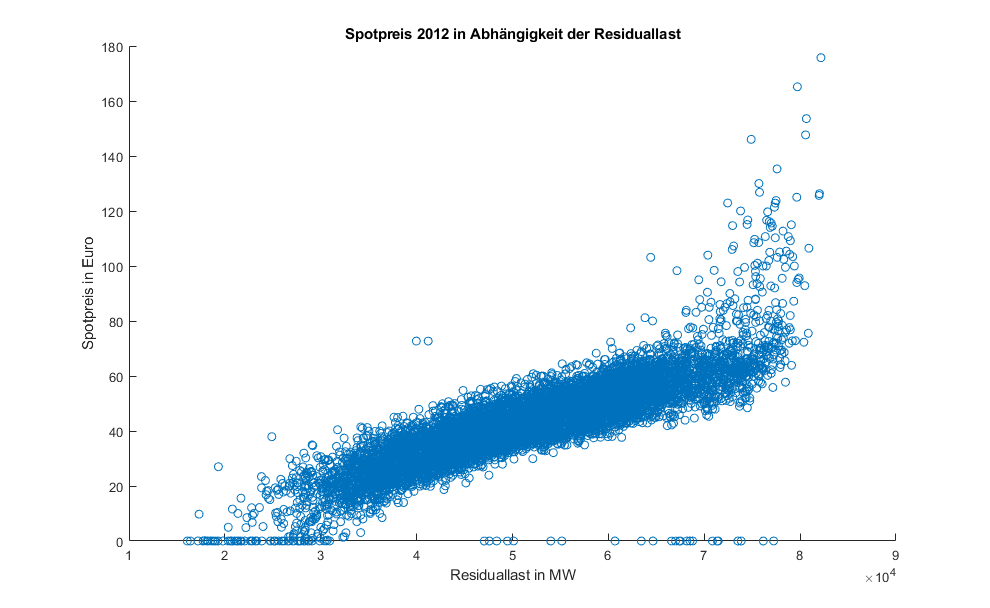
\includegraphics[width=12cm]{img/results/ScatterResiduallast}
		\caption{Die Abhängigkeit des Spotmarktpreises von der Residuallast, für das Jahr 2012.}
	\end{figure}
	\begin{figure}[H]
		\centering
		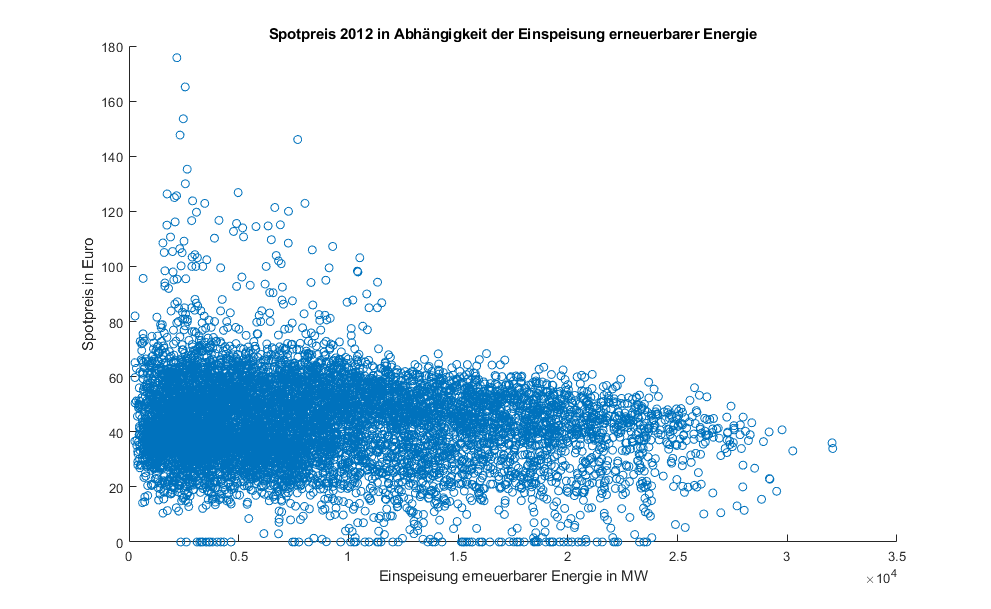
\includegraphics[width=12cm]{img/results/ScatterEinspeisung}
		\caption{Die Abhängigkeit des Spotmarktpreises von der Einspeisung erneuerbarer Energien, für das Jahr 2012.}
	\end{figure}
	\subsubsection{Aufgabe 4.1.d - Interpretation der Scatter-Plots}
	\label{sec:Ergebnisse41d}
	\begin{enumerate}
		\item Der Scatter-Plot in Abbildung 5 stellt den Spotmarktpreis, in Abhängigkeit der Netzlast dar.\newline
		Umso weiter man auf der x-Achse nach rechts geht, umso höher ist die Nachfrage nach Energie. In der Abbildung ist schön ersichtlich, wie der Spotmarktpreis bei einer hohen Nachfrage steigt, während er bei einer geringen Nachfrage (auf der linken Seite der x-Achse) sinkt.
		\item In Abbildung 6 ist der Spotmarktpreis, in Abhängigkeit der Residuallast dargestellt.\newline
		Analog zur Interpretation von Abbildung 5 ist auch in Abbildung 6 ein Zusammenhang zwischen der Nachfrage nach Energie und dem Spotmarktpreis ersichtlich. In Abbildung 6 ist dieser Zusammenhang sogar noch deutlicher sichtbar, da der unberechenbarere Faktor "erneuerbare Energien" nicht in die Berechnung miteinfließt und nur die Preissetzung der Anbieter dargestellt wird.
		\item Abbildung 7 stellt den Spotmarktpreis in Abhängigkeit der Einspeisung erneuerbarer Energie dar.\newline
		In diesem Diagramm ist ersichtlich, dass der Spotmarktpreis bei einem großen Angebot an Energie sinkt. Bei einem begrenzten Angebot, wie es links in der Abbildung der Fall ist, ist der Spotmarktpreis hoch. Bei einem großen Angebot sinkt der Preis dementsprechend.
	\end{enumerate}
	Zusammenfassen kann man sagen, dass sich die Ergebnisse mit unseren Erwartungen decken. Es ist ein allgemeiner Zusammenhang zwischen der Nachfrage nach Energie und dem Spotmarktpreis ersichtlich.\newline Sobald eine hohe Nachfrage besteht, die fluktuierende Einspeisung von dargebotsabhängigen Erzeugern jedoch gering ist, steigt der Spotmarktpreis.\newline
	Besteht eine geringe Nachfrage während die Einspeisung durch erneuerbare Energien hoch ist (z.B. zur Mittagszeit im Sommer), sinkt der Spotmarktpreis.
	\newpage
	\listoffigures
\end{document}